\chapter{Discussion}
% TODO: reflect on the work done; analyze the choices made etc. as objectively
% as possible

In this chapter, we discuss the work completed towards reconstructing a 3D mesh of the human body and outline suggestions for making a comprehensive implementation. We also analyze the choices made and the operability of different parts of the system. Finally, we conclude by reviewing the major achievements of this thesis, while examining problems in planning and conducting the research.

The approach we deem the most promising is illustrated in its current form in figure~\ref{fig:steps}.

\begin{figure}
    \centering
    
    \begin{minipage}{0.39\textwidth}
        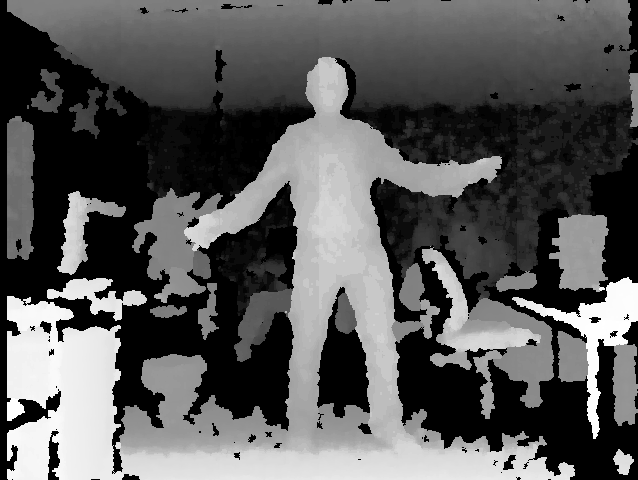
\includegraphics[width=\textwidth]{depth}
    \end{minipage}
    \begin{minipage}{0.60\textwidth}
        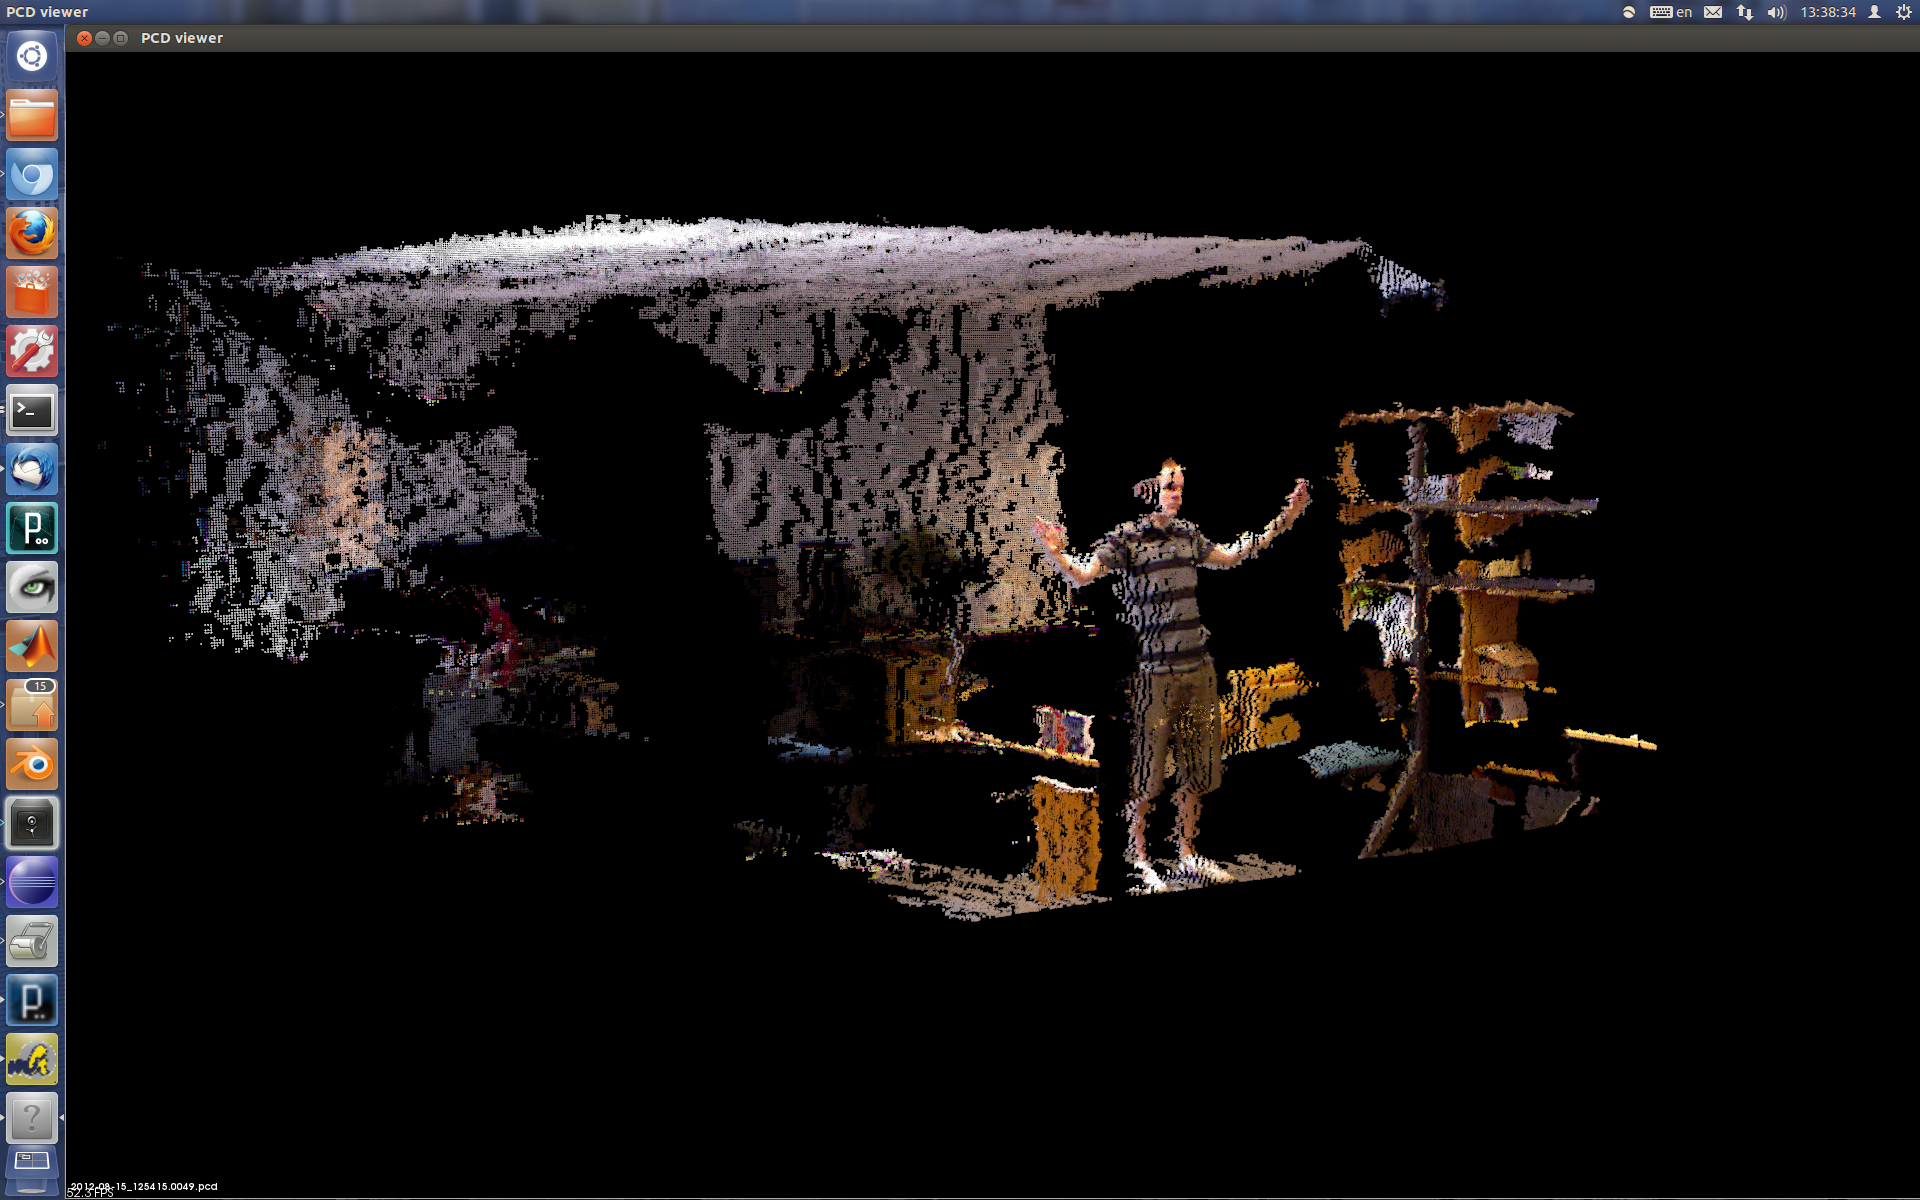
\includegraphics[width=\textwidth]{pcd-plain}
    \end{minipage}

    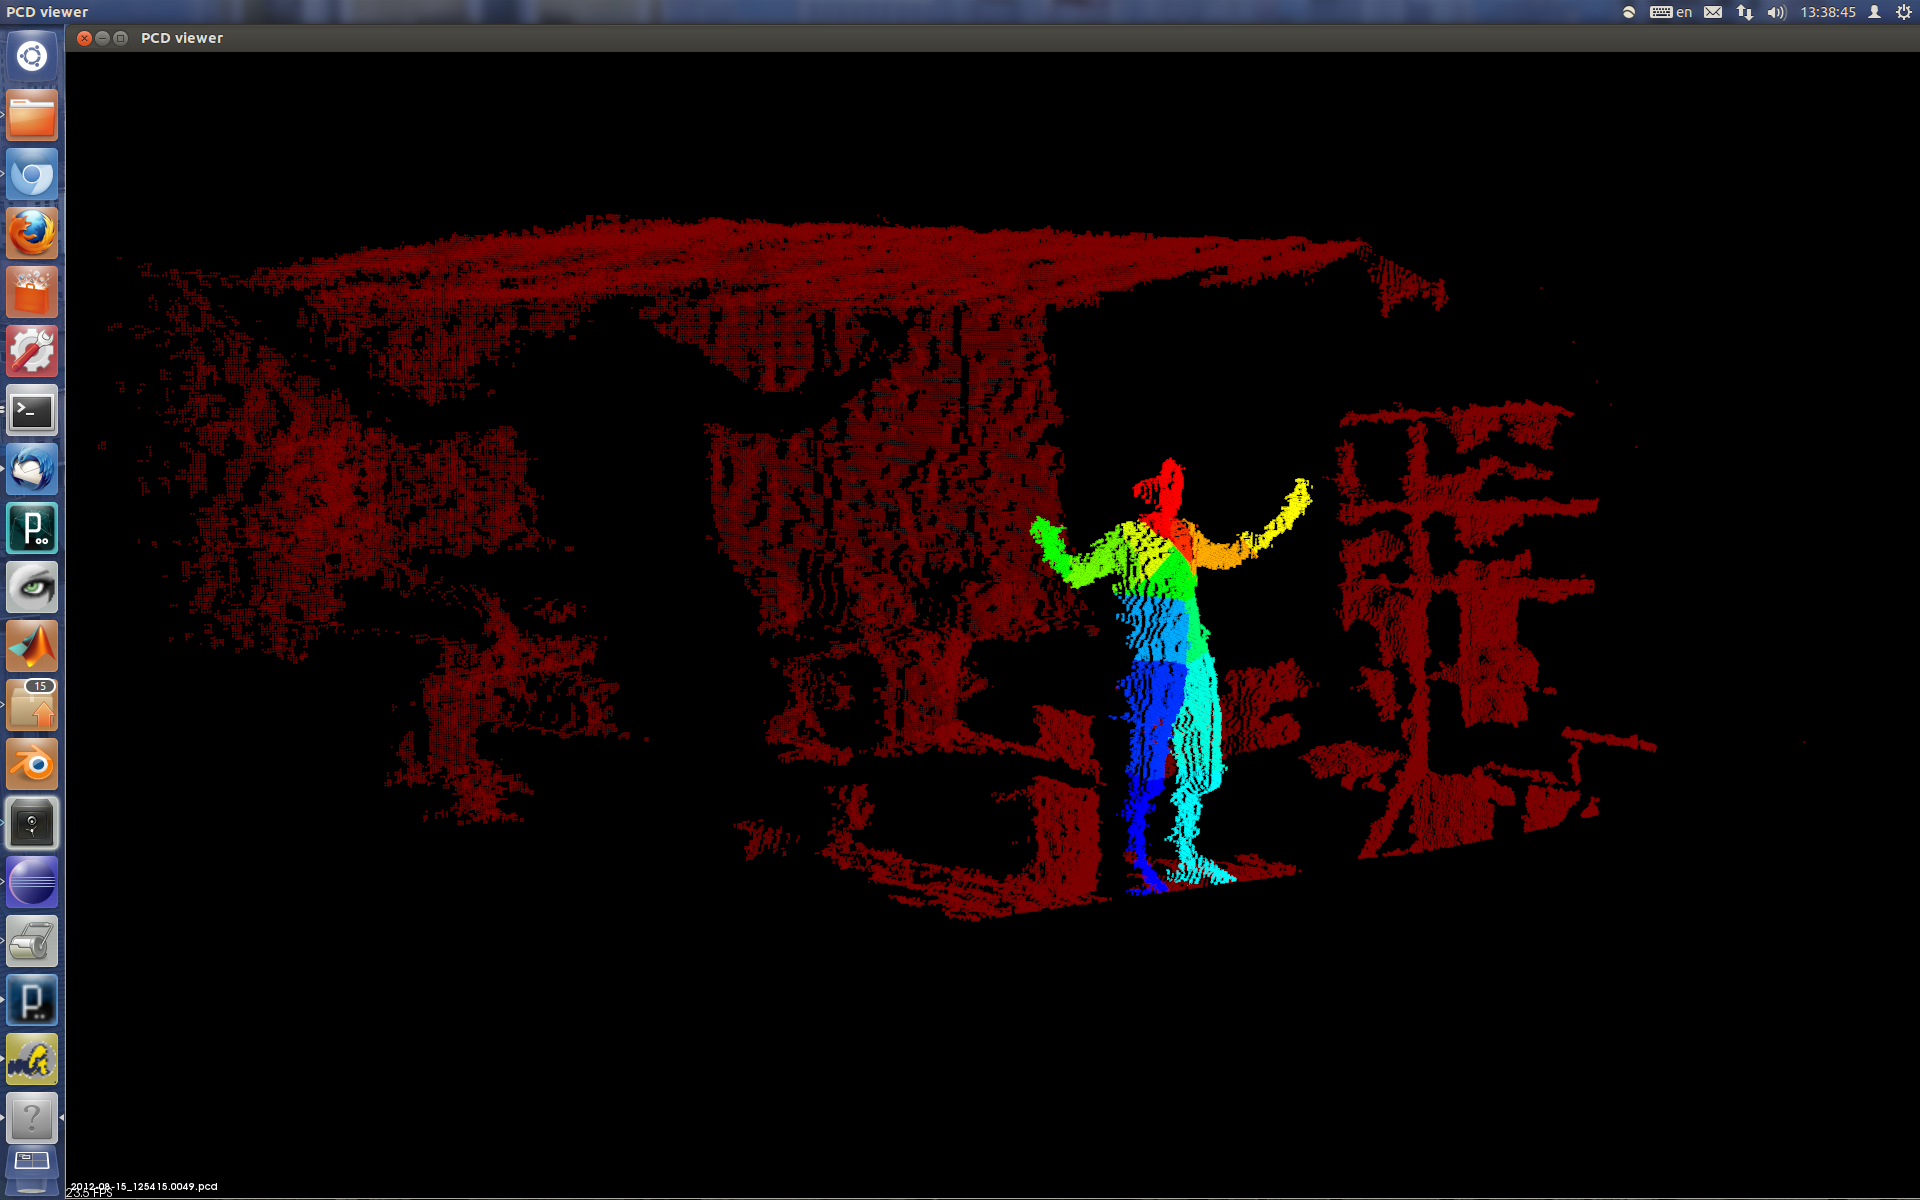
\includegraphics[width=\textwidth]{pcd-segmented}
    
    \begin{minipage}{0.56\textwidth}
        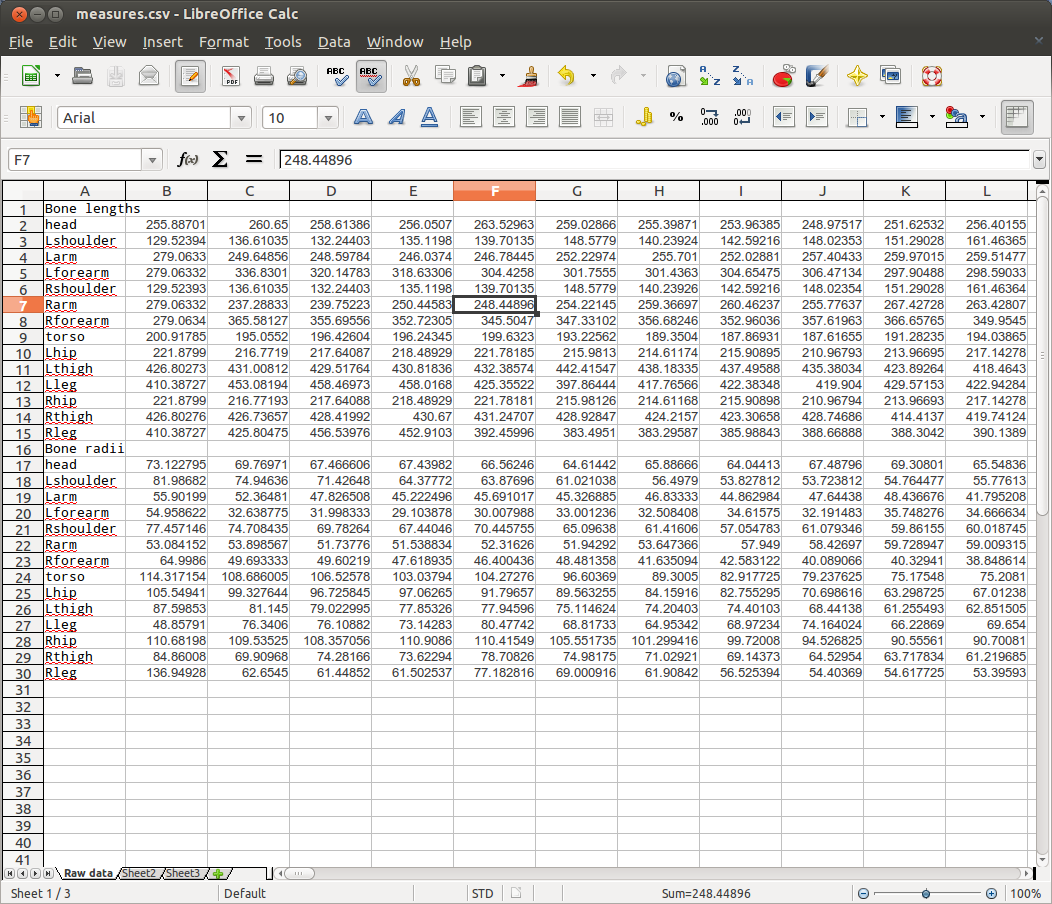
\includegraphics[width=\textwidth]{spreadsheet1}
    \end{minipage}
    \begin{minipage}{0.43\textwidth}
        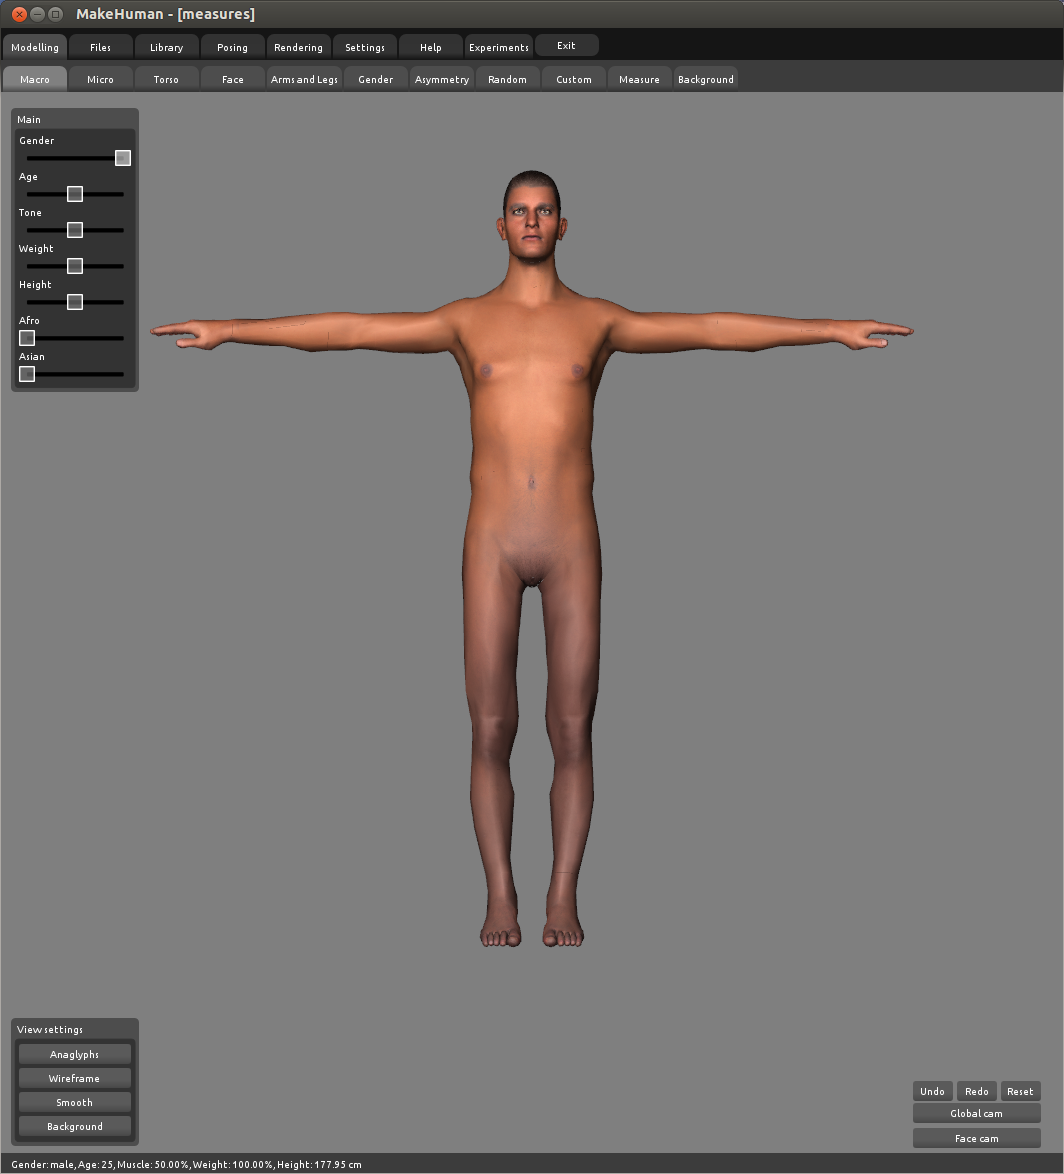
\includegraphics[width=\textwidth]{measured-hannu}
    \end{minipage}
    
    \caption{The steps to reconstruct a MakeHuman model of the user. 1) Depth data is received from Kinect. 2) The depth measurements are converted to a point cloud. 3) The point cloud is segmented and each body part is measured. 4) The measurements are copied to a spreadsheet and used to compute MakeHuman measurement values. 5) The values are manually input into MakeHuman, and a model is created.}
    \label{fig:steps}
\end{figure}

\newtopic

The scope of our work was human body reconstruction, and we chose a Microsoft Kinect for Xbox 360 as the hardware sensor to be used. We tried using three different driver libraries for the hardware, and decided OpenNI and NITE to be the most suitable. This choice was based on impressions gained through brief testing---a further assessment would be required to objectively decide whether OpenNI is truly better than Microsoft Kinect SDK for the task. We outline the known differences in section~\ref{literature.drivers}. However, we concede that the accuracy of skeleton tracking is important, and our knowledge of it is inexact. Ideally, we would have utilized an open source skeleton tracking system that has been thoroughly tested---if one existed.

The choice of sensor dictated that work would go on using 3D point data. Image-based reconstruction deserves to be researched, too, but requires a better RGB sensor than the one Kinect has. In principle, using depth information should make reconstruction very easy, but in practice the inaccuracy and noise cause difficulties. This became apparent as work progressed.

Our raw data, then, comprised point clouds gathered using OpenNI, with users segmented from the background and their skeletons tracked by NITE.

We decided that reconstruction should become easier if we further segment the point cloud into sub-clouds containing points of a single body part. The exact manner this was done was a nearest-neighbor search; each point is assigned to the nearest bone. This makes our approach heavily dependent on the skeleton data and vulnerable to errors therein. Moreover, the amount of bones in the NITE skeleton is small, yielding few body parts. On the other hand, better segmentation would require more a priori knowledge---perhaps a skeleton with more bones or a machine learning algorithm with a database of segmented bodies. Consequently, we could not realistically get significantly better body part segmentation given the resources available.

Another consideration is whether a method that doesn't rely on body part segmentation would be feasible. This is actually the case with the method \citet{weiss2011home} employ, with notable success. Using an existing template mesh, posing it similarly to the user and optimizing according to the point cloud is an approach worthy of consideration. Nonetheless, we chose not to extend our work in this direction, as the computational difficulty of such approaches has been great. We chose to strive for a system simple enough to work in real time instead.

At this point, we branched our efforts to try different approaches. As documented in sections \ref{literature.alignment} and \ref{approach.alignment}, we researched point cloud alignment methods and their suitability for fitting point clouds from subsequent frames together. Our literature review and brief tests showed that most methods available are slow, which left us with the fast GPU implementation of ICP included in PCL. Another approach suggested and prototyped by Klaus Förger avoided point cloud alignment, and depended on the skeleton for estimating the relative position of the points. The hypothesis is that given enough data, errors can be averaged out. Unfortunately, the accumulated point clouds seemed noisier than we hoped for in our preliminary tests. Having seen the problems related to point cloud alignment and accumulation, we decided to avoid working with them directly. After all, we could just use Kinfu for mesh reconstruction and gain the benefits of using ICP.

We found two alternative approaches for utilizing Kinfu. One was suggested by \citet{charpentier2011accurate}, and we describe our attempt in section \ref{approach.autorig}. The approach worked quite well, but is clearly not possible in real time. Another approach we had high hopes for was running Kinfu in parallel for each body part. Disappointingly, this approach did not work at all. Our attempts to find a workable approach with Kinfu turned out to be futile.

Two other approaches for mesh reconstruction were also researched. These methods can work on a single frame, and thus do not rely on point cloud alignment. One was the simple ``cylinder man'' method described in section~\ref{approach.cylinders}, which was easy to implement and worked well---but whose accuracy was not nearly enough for us. Ways to improve on this basic idea were contemplated, but no great ideas were found. Finally, we tried to utilize MakeHuman to create believable human shapes by taking measurements of the point clouds and changing parameters accordingly. This approach turned out to be the most promising---it is suitable for real-time computation and the humans created with MakeHuman look convincing.

Unfortunately, we did not reach a working complete system. Adapting measurements made from segmented point clouds to the MakeHuman ones is not entirely straightforward. Measuring many different people using Kinect and manually testing different ways of generating MakeHuman parameters from the measurements would be beneficial. Regrettably we had no time to do that properly. We did create a spreadsheet for calculating MakeHuman parameters from raw measurement data, but many of the decisions we had to make were unfounded. This is because the correspondence between the NITE skeleton and the MakeHuman model is unknown. In retrospect, this is one reason depending heavily on the skeleton tracking is problematic, and should have been considered more carefully. % Moreover \fixme{TODO: what was i thinking here?}

With the spreadsheet we have a way to create an avatar with MakeHuman, albeit manual work is required. Textual output from our measurement application needs to be copied into a worksheet. Then parameter values are automatically computed (though using dubious methods), and they need to be manually copied into MakeHuman. For posing and animating the generated mesh, exporting to Blender is required. This amount of manual work is unacceptable when compared to our original goal---but negligible when compared to the approach using Kinfu and automatic rigging as described in section~\ref{approach.autorig}.

All in all, we have outlined a method of creating a MakeHuman model of the user. We have implemented an application for making preliminary measurements. These measurements should be used to calculate MakeHuman parameters; we have briefly tried this, but more research is needed to find a well-defined, well-founded relation between the two sets of values. We have reimplemented the MakeHuman system of modifying a base mesh according to parameters. Therefore, if automatic parameter calculation were properly researched and implemented, we would have all the parts in place for a complete 3D body reconstruction system. The system would be able to optimize the body shape of a template in real time while rendering the model in a static pose. The model could be saved in the MakeHuman file format and exported to Blender for posing and animation.

Admittedly, even if this described system were completed, relying on an external program and manual work for animation is unhoped-for. Skeletal animation could be implemented, of course. Similarly, no implementation of texturing was made, even though texture is very important for an avatar. Our original intent was to implement texturing, too, and we discuss some of our plans for it in section~\ref{approach.texturing}. That said, we left even the mesh reconstruction in an unfinished state as we lacked the resources to finish. Not working on texturing and skeletal animation is therefore a justifiable decision.

Looking back, many significant decisions were made. They had to be made, as the space of all possible approaches is too large to handle. We tried to justify every choice, and most still seem to be good ones. Some decisions have lead into problems later on, such as deciding to depend on the skeleton that NITE creates---but in that case, doing anything at all without the skeleton would have been difficult. The greatest barrier stopping us from implementing a working system was that we looked at parallel approaches to the same problem, instead of directly picking the most suitable one. Indecisiveness was a worse problem for us than the decisions themselves. On the other hand, the approach we expected the most from turned out to be the least workable---it is difficult to say which approach works in advance.

\section{Future work}

Given the nature of this thesis, plenty of opportunities for further research exist.

The approach of automatically creating a MakeHuman model described in section~\ref{approach.makehuman} was left unfinished. The system could be finished by finding proper correspondences of a point cloud and MakeHuman parameters. Ideally research should be made to see how actual measures of the body (such as forearm length and waist circumference) can be best approximated from point clouds. Furthermore, the relevant MakeHuman targets should be chosen and their effect determined so that their required weights can be directly computed.

The body part segmentation method portrayed in section~\ref{approach.segmentation} was a limiting factor in our work. Especially, finding more parts than we currently have would be beneficial. For example, discerning hand from forearm, foot from leg and neck from head would make measurements more accurate.

We considered texturing methods and discuss them in section~\ref{approach.texturing} but never tried implementing them. If a reconstruction system is later otherwise completed, texturing should also be implemented.

Things we experimented on but did not investigate in depth include the point cloud accumulation approach described in section~\ref{approach.accumulation} and the parallel Kinfu approach depicted in section~\ref{approach.parallel}. The point cloud accumulation method needs research on how a mesh can be reconstructed from the collected data. The parallel Kinfu approach might work better if visual features were considered instead of or in addition to geometric features. Testing this in practice will be easy if the source code to Kintinuous is released, as Kintinuous already supports three different tracking methods \citep{Whelan12rssw}.

% also: animation with the makehuman approach


\section{Conclusion}

The major accomplishments of this thesis are threefold in regard to human body reconstruction using depth camera data.

Firstly, we conducted a review of the subject matter, including existing systems and related research. In chapter~\ref{literature}, we described the most relevant areas of research in terms of what should be considered when designing a system for 3D reconstruction of the human body. We also encountered and identified the major problems that must be solved in order to create a working system.

Secondly, we suggested different valid approaches in chapter~\ref{approach}. We described each approach in terms of how the problem can be divided into sub-tasks and determined requirements for their implentations. We also analyzed possible problems with each approach and recommended the one we deemed most promising.

Thirdly, we made prototype implementations for many of the tasks described, as described in chapter~\ref{approach}. These implementations helped us further understand the tasks and problems that must be solved. They also provide a useful basis for further work on a complete human body reconstruction system.

\newtopic

Ultimately, this research did not meet its original goal---a complete human body reconstruction system that works in real time. Various causes contributed to this result. Fundamentally, the difficulty of achieving the chosen research goal was seriously underestimated. Our lack of previous knowledge of the subject matter was the primary reason for this. Unfortunately, there was little existing expertise in relevant research topics in the Department of Media Technology, and instruction during the research was lacking. Therefore, it took us long to realize our mistake.

Still, we have made a promising start in the research---the error was mostly in choosing the scope to fit the limited resources of a Master's thesis. Scoping the research appropriately was made difficult by the broadness of the subject. Any given task requires a broad understanding of different research areas, which had to be gained first. We also made the error of focusing on finding a lot of different ideas---while neglecting validation of their feasibility before committing to working on them.

All things considered, we made good groundwork by investigating, planning and partially implementing a system for human body reconstruction, while our original goal was not completely met.
